%!TeX root=../thesis.tex
%("dica" para o editor de texto: este arquivo é parte de um documento maior)
% para saber mais: https://tex.stackexchange.com/q/78101/183146

\chapter{Work Plan}
\label{chap:work_plan}
%%%%%%%%%%%%%%%%%%%%%%%%%%%%%%%%%%%%%%%%%%%%%%%%%%%%%%%%%%%%%%%%%%%%%%%%%%%%%%%%

This PhD research started at University of São Paulo (USP) in late 2020.
Besides the challenges of the COVID-19 pandemic, the author was working in
a full-time job as \emph{principal machine learning engineer} at
\href{https://www.elo7.com.br}{Elo7} -- an experience that inspired
this research. In 2023, this PhD started being developed in a sandwich
doctorate in the Jheronimus Academy of Data Science (JADS) in the Netherlands.
Since 2024, the author has been employed as a \emph{scientific programmer}
in the \href{https://marit-d.eu/}{MARIT-D European project}.

This chapter presents a work plan to execute the research methodology
from \cref{chap:research_methodology}. The timeline considers this PhD
is not a full-time activity. \Cref{tab:work_plan} accounts time to:
%------------------------------------------------------------------------------%
\begin{itemize}
  \item execute each step of the methodology,
  \item submit publications about the results of each phase of the methodology, and
  \item write the thesis for final submission.
\end{itemize}
%------------------------------------------------------------------------------%

%------------------------------------------------------------------------------%
\begin{table}[b!]
  \centering
  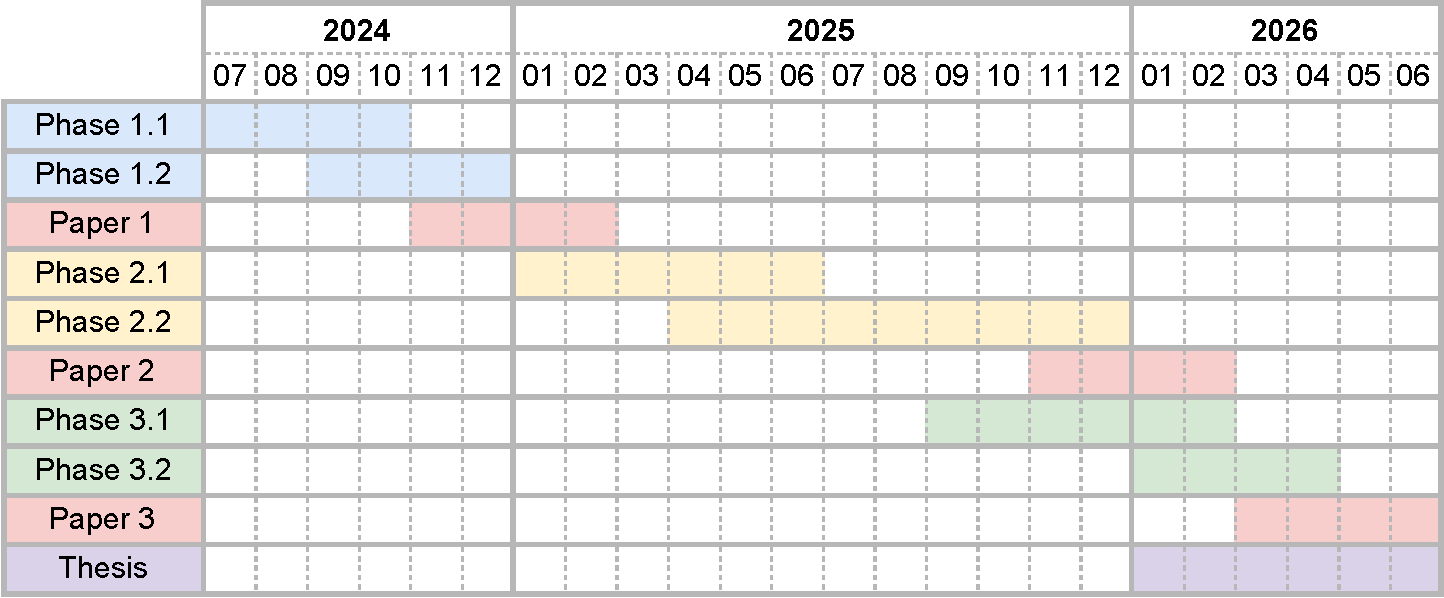
\includegraphics[width=0.85\linewidth]{tables/Timetable.pdf}
  \caption[%
    Work plan%
  ]{%
    \emph{Work Plan}. The timetable summarizes the expected number
    of months to complete the research methodology introduced in
    \cref{chap:research_methodology}. Each line represents a task,
    each column represents a month. Lines and cells are color-coded
    according to \cref{fig:research_methodology}.
  }
  \label{tab:work_plan}
\end{table}
%------------------------------------------------------------------------------%